\chapter{Introduction}
    
\fcolorbox{black}[HTML]{E9F0E9}{\parbox{\textwidth}{%
\noindent \textbf{Learning goals}\\
The junior-colleague
\begin{enumerate}[nolistsep]
\item can describe what Spring is
\item can describe what Spring Boot is
\item can explain what a three-tier application is
\item can identify the three layers in a Spring Boot application
\item can explain the responsibilities of the layers in a Spring Boot application
\item can explain the architecture of a Spring RESTful web application
\item can explain what a DTO is
\item can explain what an entity-object is
\item can explain what dependency injection is
\item can explain what a Spring bean is
\item can explain what a Spring container is
\item can explain what a Spring Boot starter is
\end{enumerate}}}


\section{Enterprise Applications with Java}
By 1999, Java had developed a loyal following among application developers and Sun saw an opportunity to extend the language for traditional enterprise workloads. With the launch of J2EE, and another technology that was gaining prominence — the application server — enterprises now had a platform that was designed to meet their needs with capabilities for things like security, scalability and reliability.

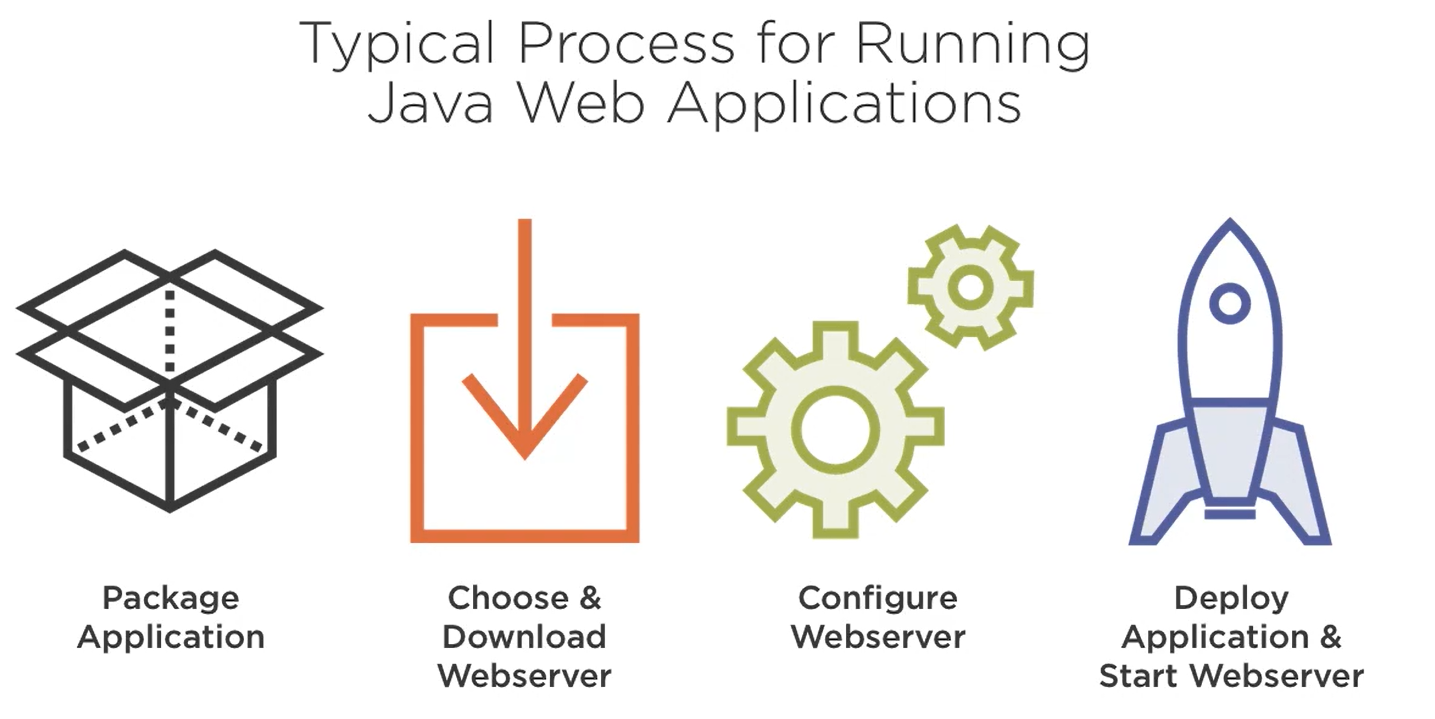
\includegraphics[width=\textwidth]{./images/chapter1/before_spring_boot.png} 

Spring came into being in 2003 as a response to the complexity of the early J2EE specifications. While some consider Java EE and its modern-day successor Jakarta EE to be in competition with Spring, they are in fact complementary. The Spring programming model does not embrace the Jakarta EE platform specification; rather, it integrates with carefully selected individual specifications from the traditional EE umbrella. Spring started as a lightweight alternative to Java Enterprise Edition. Rather than develop components as heavyweight Enterprise
JavaBeans (EJBs), Spring offered a simpler approach to enterprise Java development, utilizing dependency injection and aspect-oriented programming to achieve the capabilities of EJB with plain old Java objects (POJOs).
But while Spring was lightweight in terms of component code, it was heavyweight in terms of configuration. Initially, Spring was configured with XML (and lots of it).
It provides everything you need to create Java enterprise applications. Spring offers the flexibility to create many kinds of architectures depending on an application’s needs. As of Spring Framework 6.0, Spring requires Java 17+.

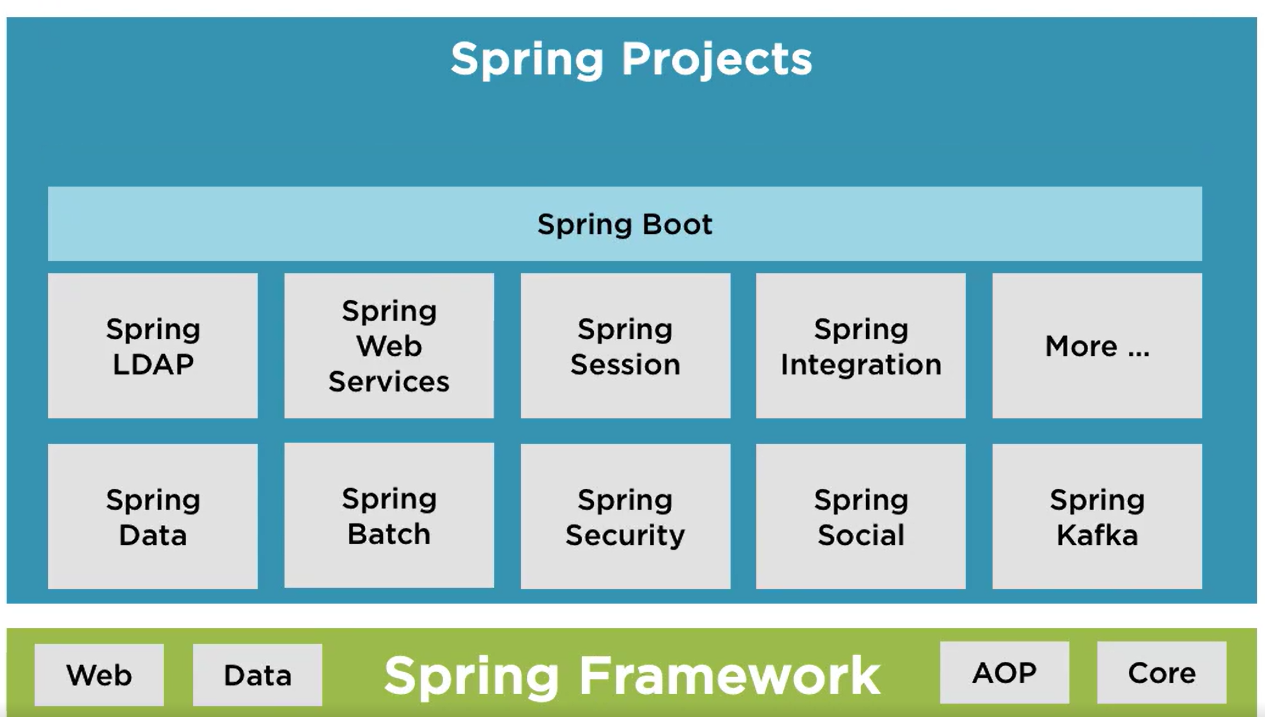
\includegraphics[width=\textwidth]{./images/chapter1/spring_framework.png} 

Spring Boot is a project that is built on the top of the Spring Framework. It provides an easier and faster way to set up, configure, and run java applications.

    
\section{What is Spring Boot?}
 
Spring Boot is an open-source Java framework to create production-ready,  standalone Spring applications. It's a robust, widely used framework. The creation of this framework was facilitated by the desire to simplify the development of applications on the popular Java EE technology stack from Oracle, which was very complex and difficult to use at the time. With very little configuration, you can create easily your first Spring Boot application.

Let's look at some advantages of Spring Boot for developers 
\begin{itemize}
\item speed up the process of creating and deploying application
\item create standalone applications with less or almost no configuration overhead
\item easy to learn framework
\item increase productivity of developers
\end{itemize}

\section{Bootstrapping a simple application}

\subsection{Using Spring Initializr}
Spring Initializr is a web application that can generate a Spring Boot project.
The url for this web application is \url{https://start.spring.io/}. You can select the necessary configuration, including the build tool, language, version of the Spring Boot framework, and any dependencies for your project. IntelliJ IDEA Ultimate provides the Spring Initializr project wizard that integrates with the Spring Initializr API to generate and import your project directly from the IDE.

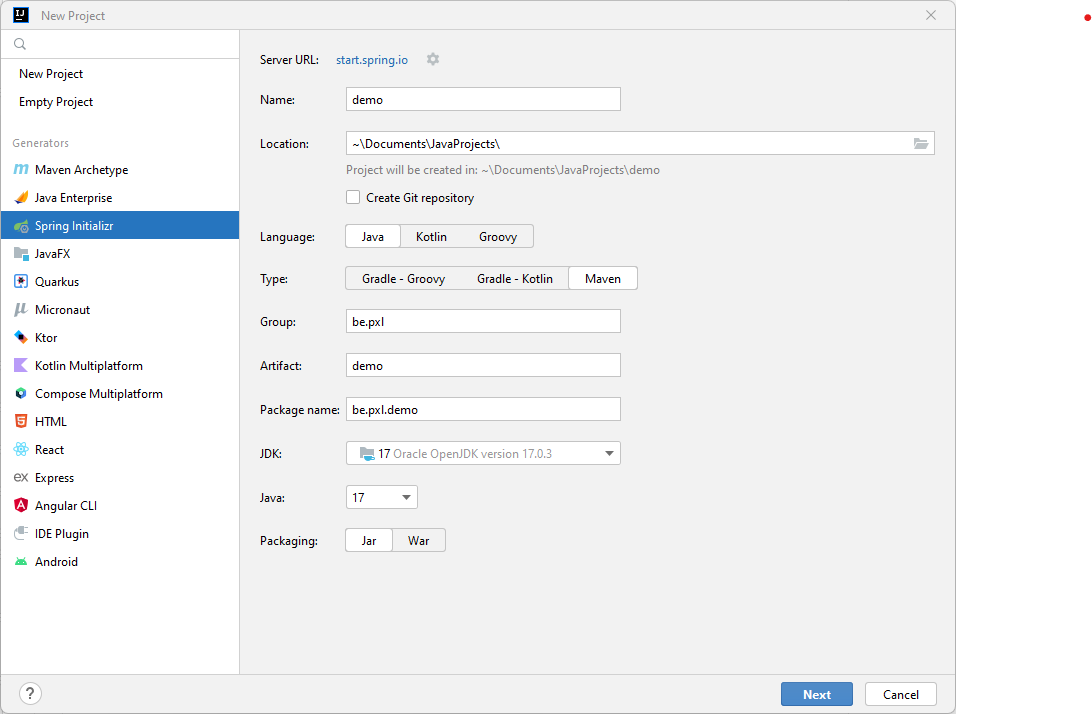
\includegraphics[width=\textwidth]{./images/chapter1/spring_initializer_intellij.png}

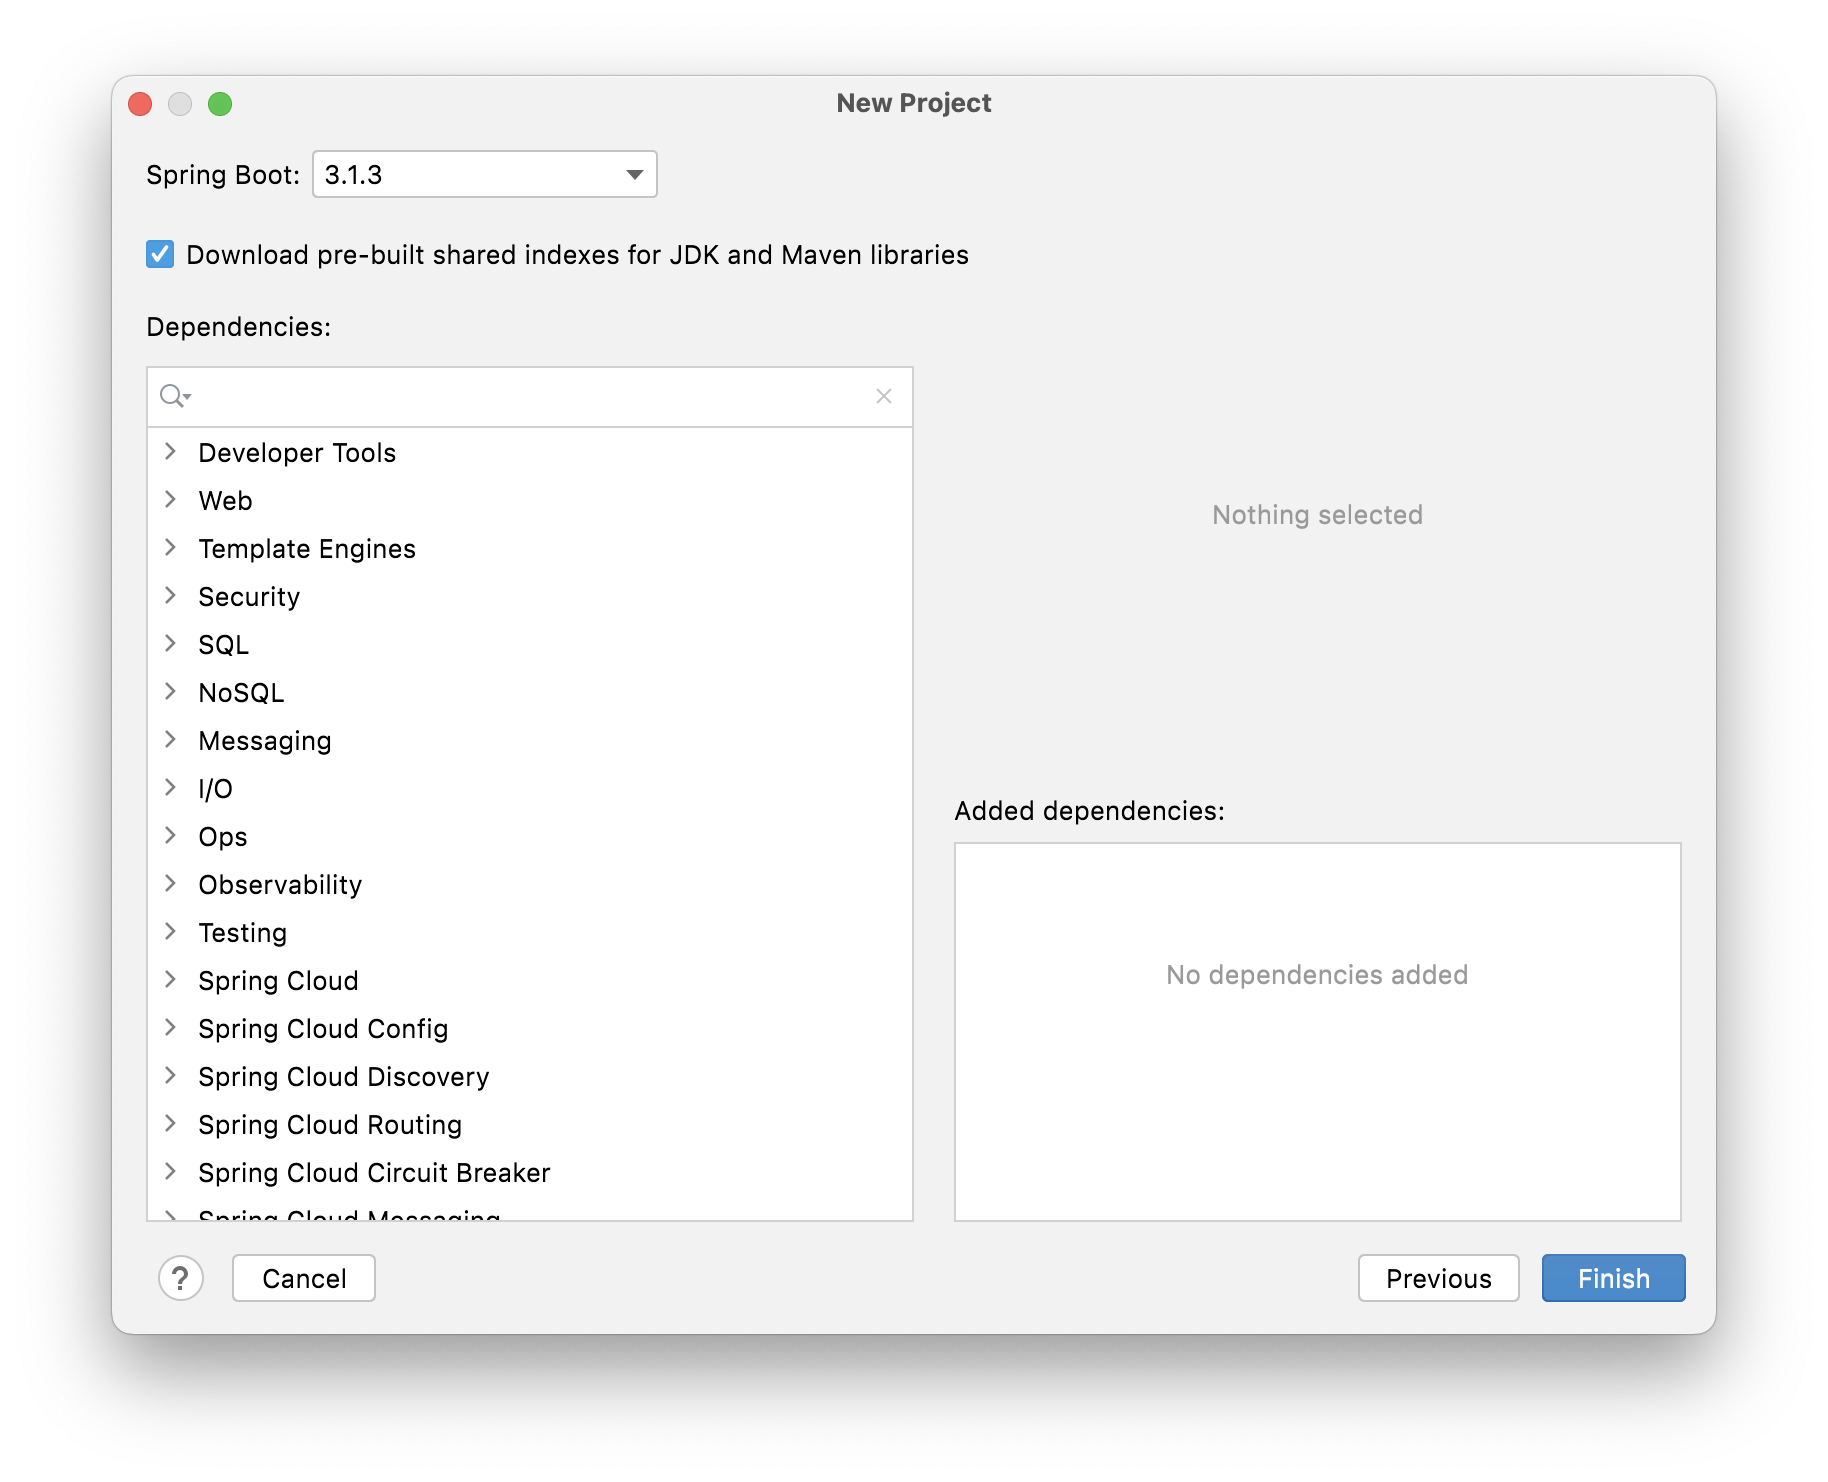
\includegraphics[width=\textwidth]{./images/chapter1/new_project.png}

We select Spring Web dependency. Spring Web uses Spring MVC. It is used for building RESTful Web Services. Spring MVC provides the annotation @RestController for classes that implement the REST endpoints.
To run a RESTful Web Service you need a web container. Spring Boot will automatically add an embedded Tomcat web container to your project. If you prefer another web container, you can update Spring Boot's configuration.
Finally Jackson is a popular third-party library for converting Java-objects to JSON and vice versa.

\begin{oefening}
Create the demo project. You can use the wizard in IntelliJ IDEA Ultimate or \url{https://start.spring.io/}.
\end{oefening}

\section{Running the demo project}

The starting point of a Spring Boot application is the class with the main-method and annotated with @SpringBootApplication.  This class can be found in the folder /src/main/java.  Spring Boot offers a lot of annotations to reduce the workload of developers.   

\begin{lstlisting}[frame=single]
package be.pxl.demo;

import org.springframework.boot.SpringApplication;
import org.springframework.boot.autoconfigure.SpringBootApplication;

@SpringBootApplication
public class DemoApplication {

    public static void main(String[] args) {
        SpringApplication.run(DemoApplication.class, args);
    }

}
\end{lstlisting}

By running the main-class you start your Spring Boot application. 

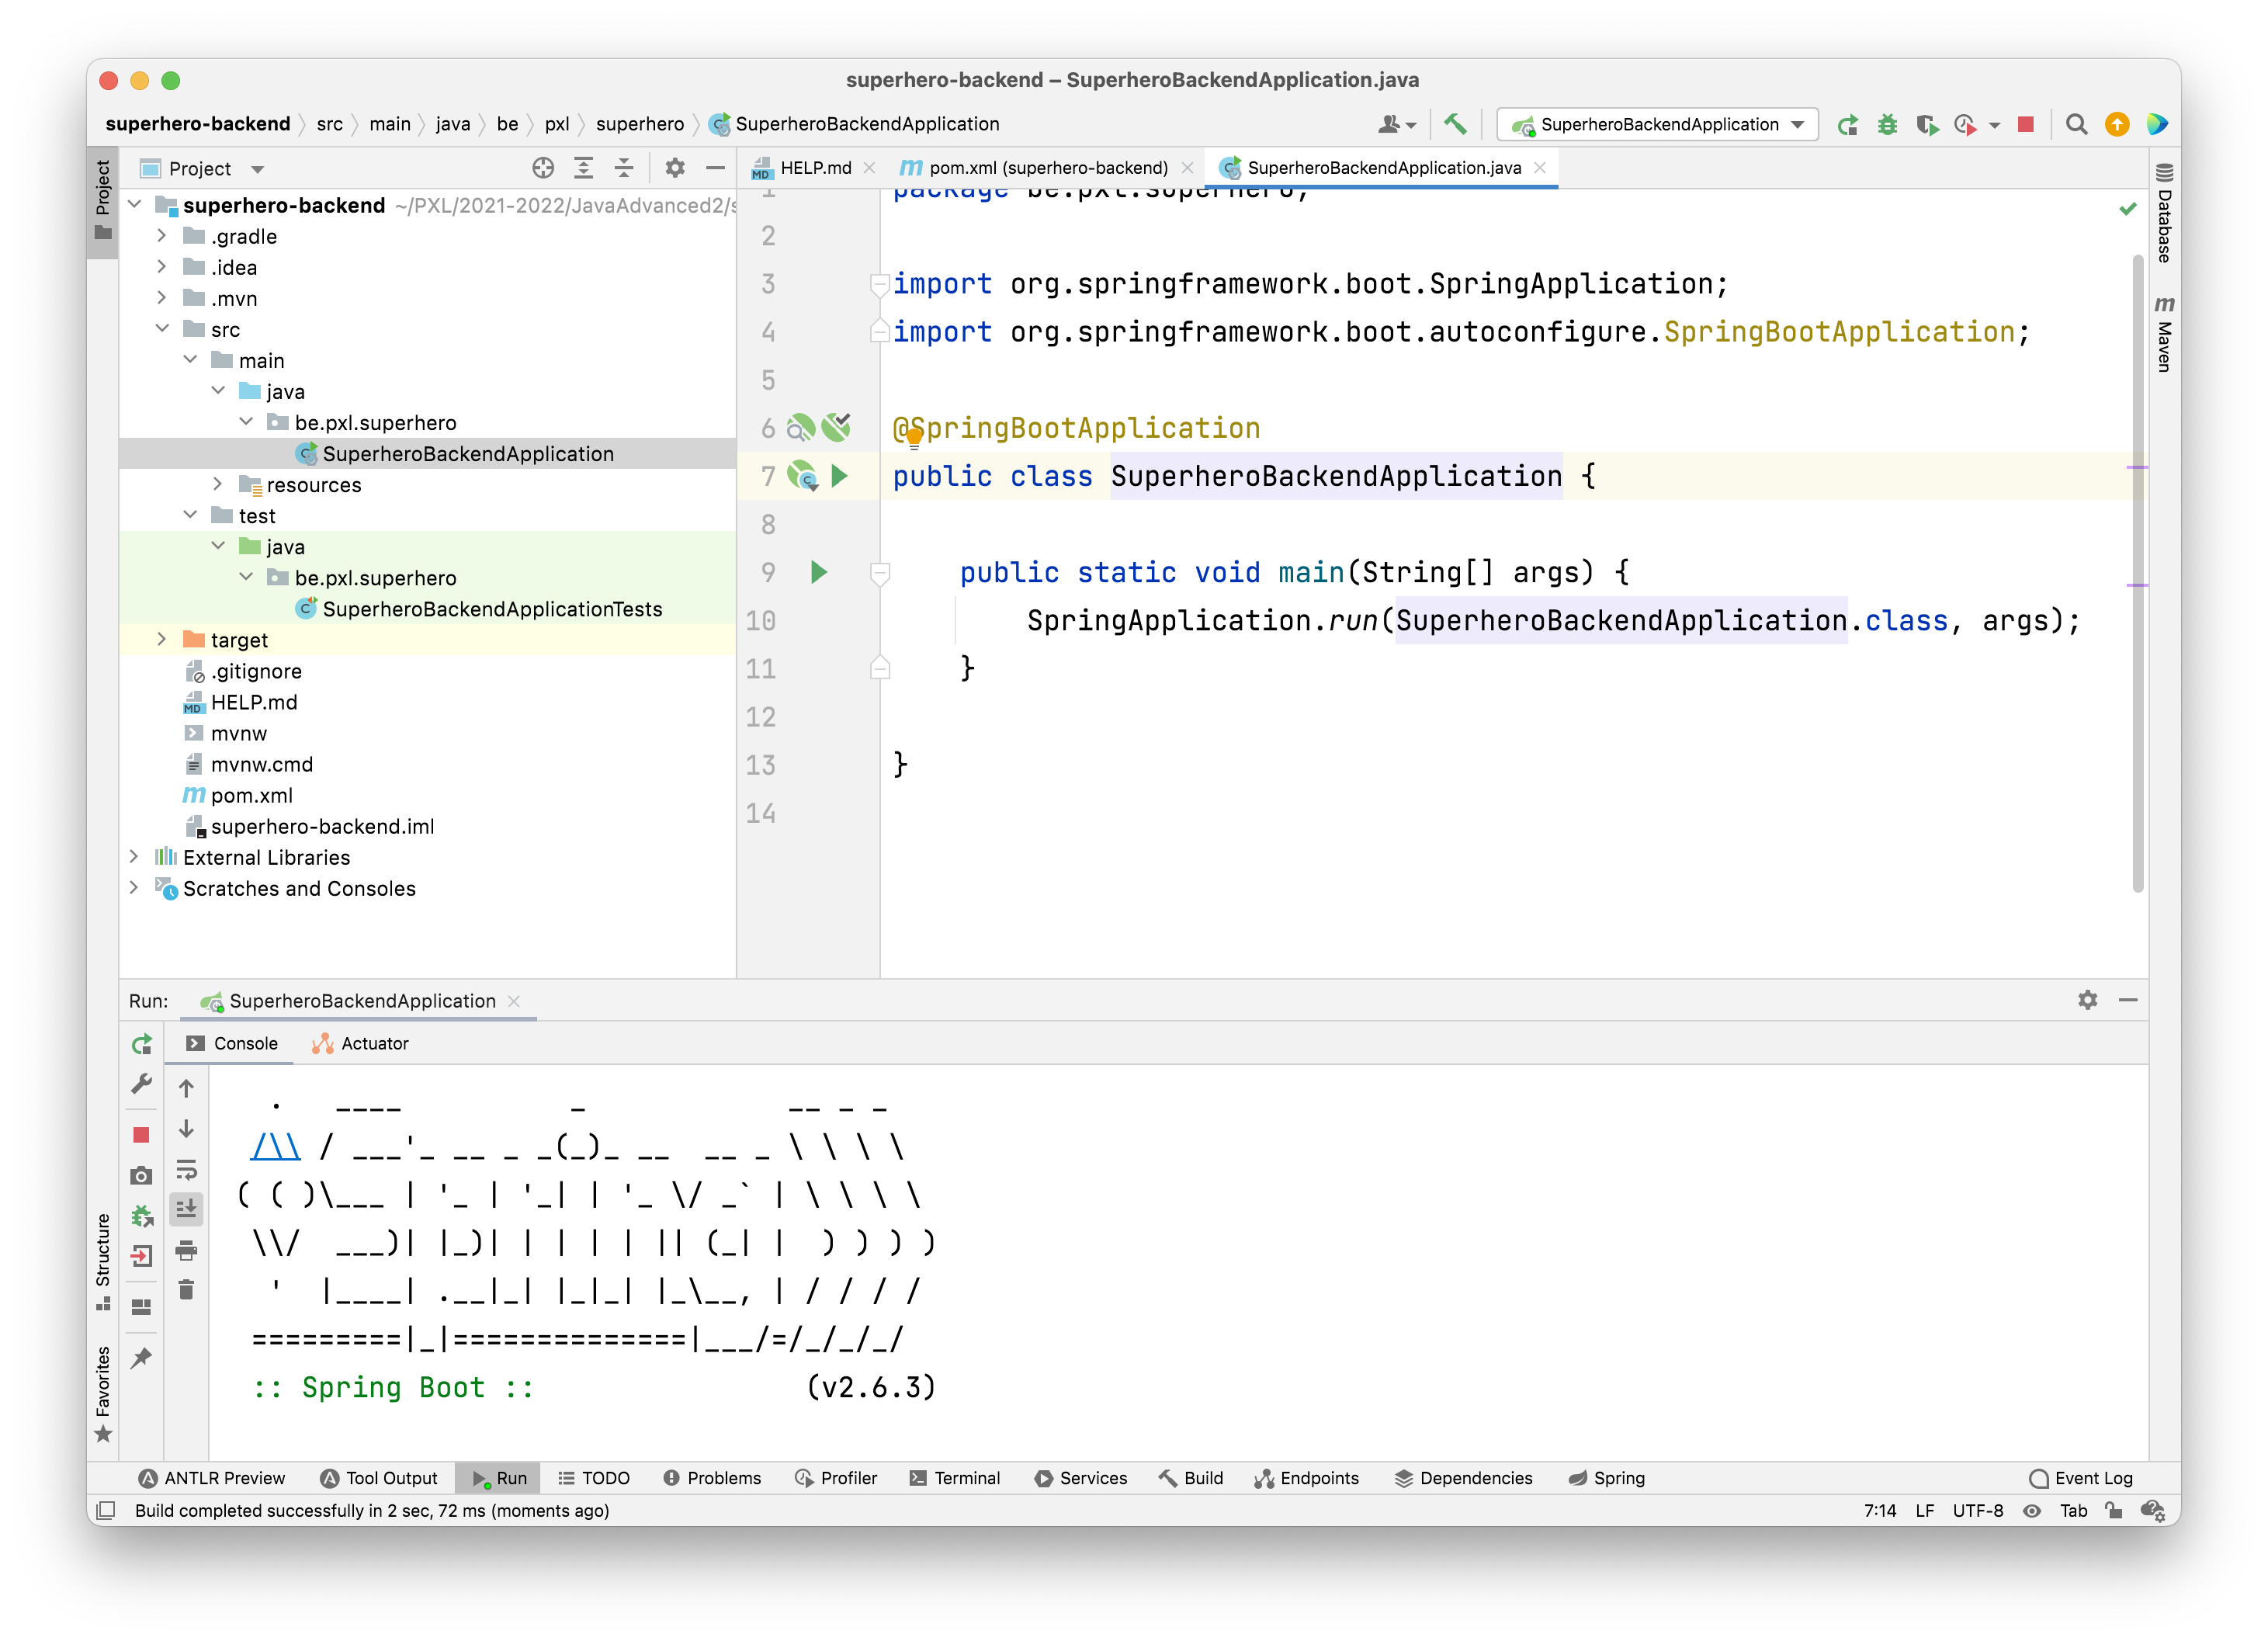
\includegraphics[width=\textwidth]{./images/chapter2/first-run.png}

Currently our Spring Boot application only shows a whitelabel error page. This error page is available when you perform a GET for URL \url{http://localhost:8080}.

\frame{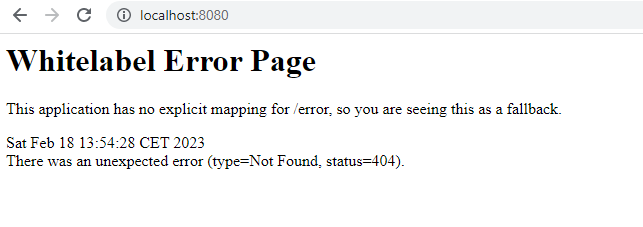
\includegraphics[width=\textwidth]{./images/chapter2/whitelabel_error_page.png}} 

Port 8080 is the default port. If this port is not available you will see an error message in Spring Boot's logging.

\begin{lstlisting}[frame=single]
***************************
APPLICATION FAILED TO START
***************************

Description:

Web server failed to start. Port 8080 was already in use.
\end{lstlisting}

The port number can be changed in the file application.properties. You have to add the property server.port here with the desired port number.

\begin{lstlisting}[frame=single]
server.port=8081
\end{lstlisting}

\subsection{The Maven pom file}

POM stands for \'Project Object Model\'. It is an XML representation of a Maven project held in a file named pom.xml. This file can be found in your project directory. The POM contains all necessary information about a project, as well as configurations of plugins to be used during the build process. We will cover Maven in chapter 3.

\begin{lstlisting}[frame=single]
<?xml version="1.0" encoding="UTF-8"?>
<project xmlns="http://maven.apache.org/POM/4.0.0" xmlns:xsi="http://www.w3.org/2001/XMLSchema-instance"
         xsi:schemaLocation="http://maven.apache.org/POM/4.0.0 https://maven.apache.org/xsd/maven-4.0.0.xsd">
    <modelVersion>4.0.0</modelVersion>
    <parent>
        <groupId>org.springframework.boot</groupId>
        <artifactId>spring-boot-starter-parent</artifactId>
        <version>3.0.2</version>
        <relativePath/> <!-- lookup parent from repository -->
    </parent>
    <groupId>be.pxl</groupId>
    <artifactId>demo</artifactId>
    <version>0.0.1-SNAPSHOT</version>
    <name>demo</name>
    <description>demo</description>
    <properties>
        <java.version>17</java.version>
    </properties>
    <dependencies>
        <dependency>
            <groupId>org.springframework.boot</groupId>
            <artifactId>spring-boot-starter-web</artifactId>
        </dependency>

        <dependency>
            <groupId>org.springframework.boot</groupId>
            <artifactId>spring-boot-starter-test</artifactId>
            <scope>test</scope>
        </dependency>
    </dependencies>

    <build>
        <plugins>
            <plugin>
                <groupId>org.springframework.boot</groupId>
                <artifactId>spring-boot-maven-plugin</artifactId>
            </plugin>
        </plugins>
    </build>
</project>
\end{lstlisting}

spring-boot-starter-parent is a starter project that provides the default configuration for spring-based applications. Here you choose the version of Spring Boot.

For large projects, managing the dependencies is not always easy. Spring Boot solves this problem by grouping certain dependencies together. These groups of dependencies are called starters. All Spring Boot starters are named following the same naming pattern. The all start with spring-boot-starter-*, where * indicates the purpose and functionality provided by the starter.

spring-boot-starter-web adds all the libraries we need to develop web components. An embedded server will be provided in the Spring Boot project. Therefore the environment where the Spring Boot project is executed does not need to have a pre-installed server. The default embedded server for Spring Boot is Tomcat. The Spring MVC framework which provides all classes for developing RESTful web services is also part of spring-boot-starter-web.

spring-boot-starter-test (with scope test) is the starter for testing Spring Boot applications with libraries including JUnit Jupiter, Hamcrest and Mockito.

